\documentclass{siproblemset}

\usepackage{multicol}
\usepackage{xcolor}
\usepackage{mathtools}
\usepackage{graphicx}

\usepackage{array}
\newcommand{\PreserveBackslash}[1]{\let\temp=\\#1\let\\=\temp}
\newcolumntype{C}[1]{>{\PreserveBackslash\centering}p{#1}}
\newcolumntype{R}[1]{>{\PreserveBackslash\raggedleft}p{#1}}
\newcolumntype{L}[1]{>{\PreserveBackslash\raggedright}p{#1}}

% SI Session Information
\course{MTH 1321}
\sessionnum{PT1}
\sessiondate{2/8/22}

% Worksheet Information
\title{Practice Test \#1}
\sections{Sections 2.1-2.8}
\withnamespace

\definecolor{darkred}{RGB}{110,0,0}

%\debugmode

\begin{document}
    \maketitle
    
    \begin{center}
        \framebox{
            \begin{minipage}{\textwidth}
                \begin{center}
                    \textbf{When completing this practice test, do your best to mimic the test environment:}
                \end{center}
                \begin{enumerate}
                    \item Do not use a calculator.
                    \item Try not to use your notes.
                    \item Time yourself, make sure you are completing the problems at a comfortable pace. Remember that you will only get 2 hours for the actual exam (with fewer questions of course).
                \end{enumerate}
                \begin{center}
                    \color{darkred}\textbf{ Please do not share this practice test with anyone else. \underline{Your} commitment to SI and reviewing material earned this, not anyone else's.}
                \end{center}
%                {\centering When you have finished the practice test, go to the following link to check your answers:\\ \color{blue}{https://baylor.box.com/s/1mo74zgq67yyy4wzz3gn22ajl3dfx87m}\\}
            \end{minipage}
        }
    \end{center}


    \frq{Determine the value of $b$ that will make $r(x)$ continuous at $x=2$. Use the definition of continuity to explain your answer.}
    $$r(x)=\begin{cases}
    x^2-b & \text{, if } x<2\text; \\
    \cos(x^2-x-2) & \text{, if } x\geq2
    \end{cases}$$

    \newpage
    
    \begin{multipartquestion}{The graph of $s(t)$ below represents a delivery driver's distance away from the company headquarters, in miles, as a function of time, in minutes.}

    \begin{center}
        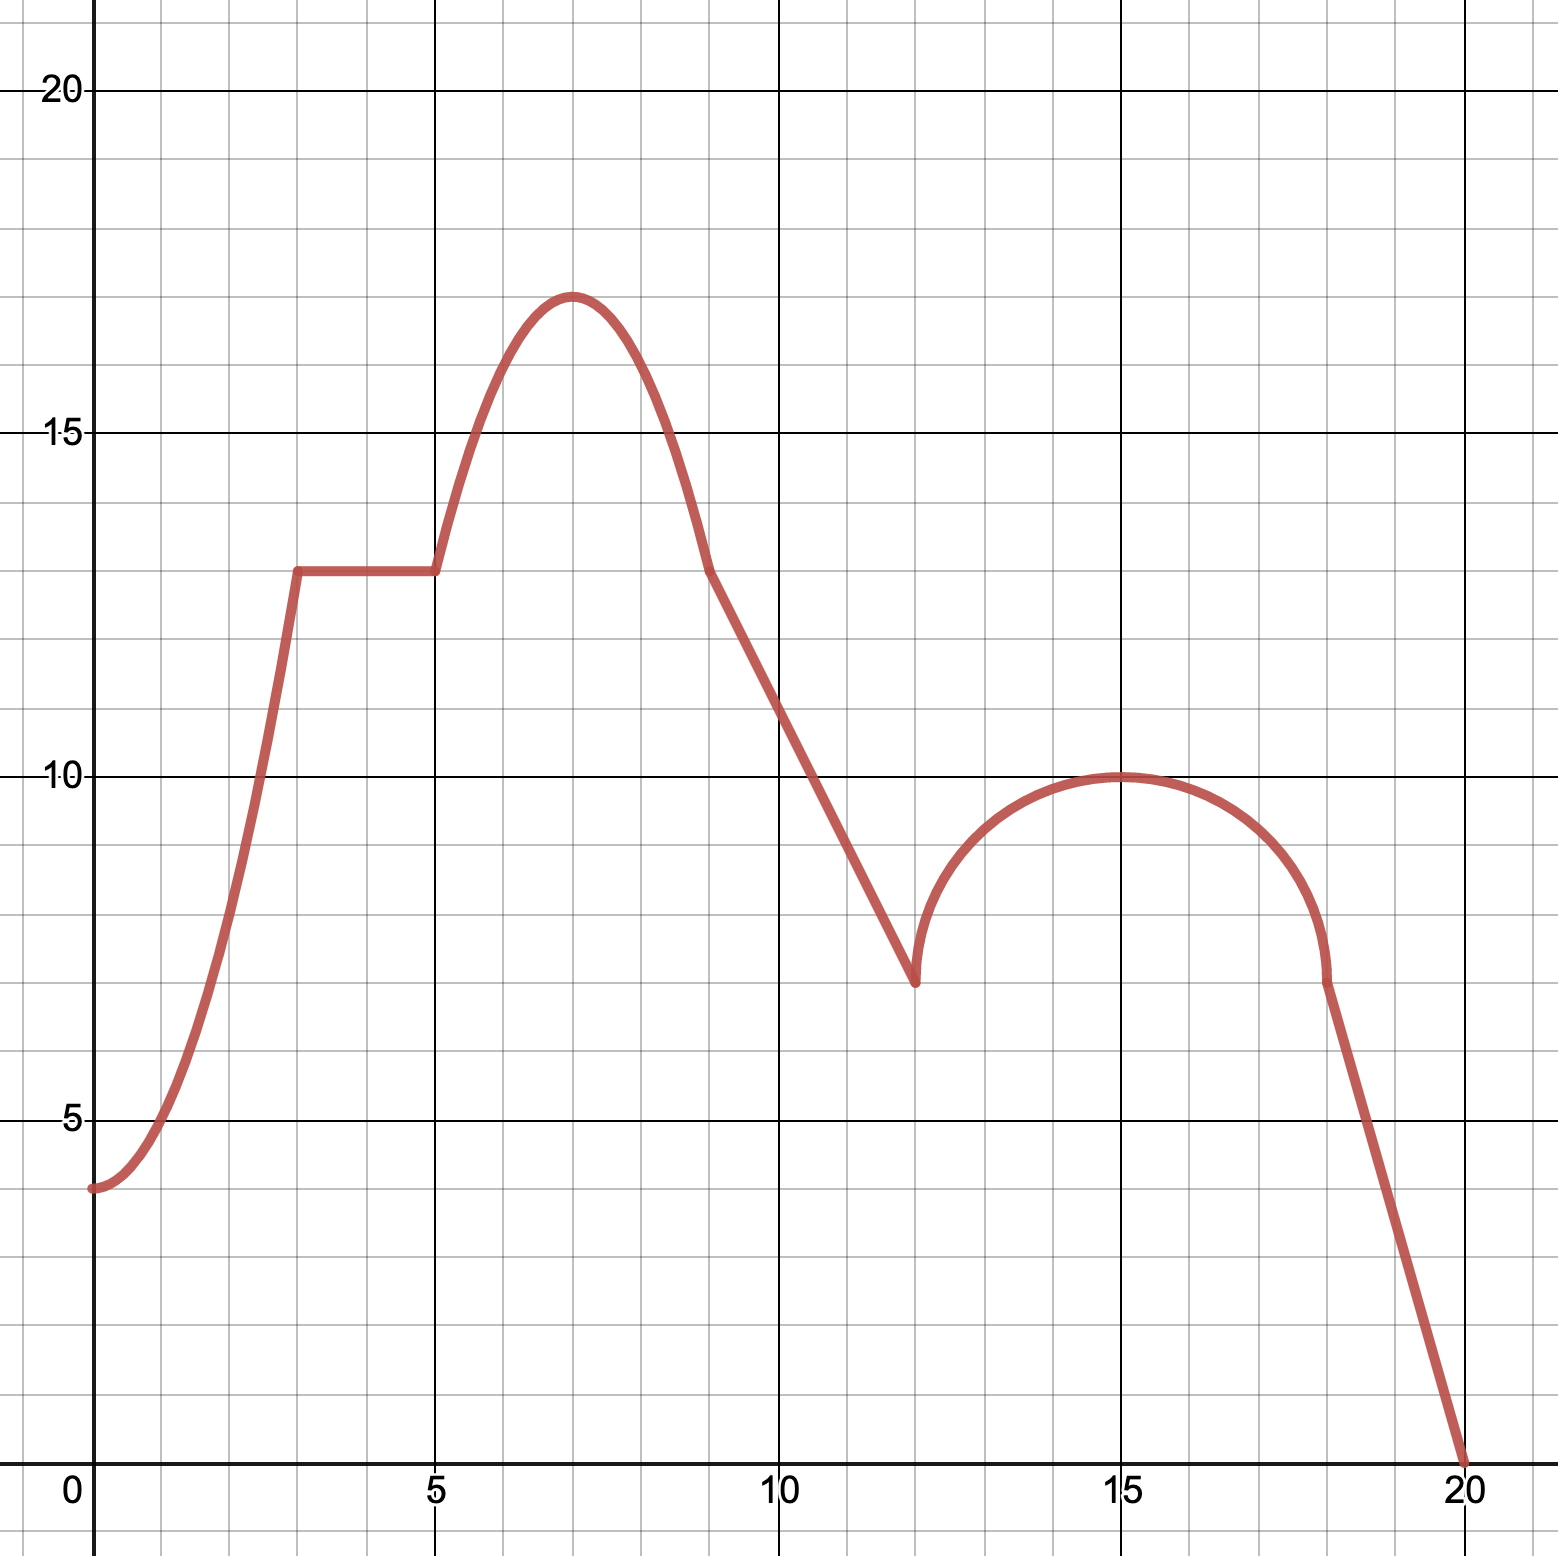
\includegraphics[width=0.5\linewidth]{img/pt1-graph1}
    \end{center}

    \frq{State two times $t_1$ and $t_2$ that the driver is moving towards the company HQ.}
    \tinysp
    \mcq[3]{At what time is the driver moving the slowest?}{
        \task $t=2$
        \task $t=7$
        \task $t=16$
    }
    \frq{Draw a line on the graph whose slope represents the instantaneous rate of change of the driver's position at time $t=17$.}
    \frq{Draw a line on the graph whose slope represents the average rate of change of the driver's position between $t=4$ and $t=7$.}
    \frq{What are the units of the function representing the rate of change of $s(t)$?}
    \tinysp
    \end{multipartquestion}

    \newpage
    
    \mcq{Given $\lim\limits_{x\to1}f(x)=4$ and $\lim\limits_{x\to1}g(x)=-3$, determine the value of the following limits. \textbf{Show at least two steps using Basic Limit Laws} and simplify your answer.}{
        \task $\lim\limits_{x\to1}(f(x)+1)^2$
        \Smallsp
        \task $\lim\limits_{x\to1}\dfrac{g(x)^2}{x-3}$
        \Smallsp
        \task $\lim\limits_{x\to1}\dfrac{\sqrt{2f(x)}}{(g(x)-1)^2}$
        \Normalsp
        \task $\lim\limits_{x\to1}\dfrac{1}{f(x)}-\dfrac{1}{g(x)}$
        \Smallsp
    }
    
    \newpage
    
    \begin{multipartquestion}{Use the table below to estimate the values of the following limits.}
    
        \begin{center}   
            \begin{tabular}{|c|C{1.2cm}|C{1.2cm}|C{1.2cm}|C{1.2cm}|C{1.2cm}|C{1.2cm}|C{1.2cm}|}
                \hline
                 \textbf{x}   & \textbf{0.9} & \textbf{0.99} & \textbf{0.999} & \textbf{1} & \textbf{1.001} & \textbf{1.01} & \textbf{1.1} \\ \hline
                \textbf{f(x)} &     12.9     &     12.99     &     12.999     &            &     13.001     &     13.01     &     13.1     \\ \hline
                \textbf{g(x)} &     6.9      &     6.99      &     6.999      &            &     -7.001     &     -7.01     &     -7.1     \\ \hline
                \textbf{h(x)} &      64      &      256      &      1024      &            &      1024      &      256      &      64      \\ \hline
                \textbf{j(x)} &      2       &      20       &      200       &            &     2.001      &     2.01      &     2.1      \\ \hline
                \textbf{k(x)} &     3.9      &     3.99      &     3.999      &            &     5.001      &     5.01      &     5.1      \\ \hline
            \end{tabular} 
        \end{center}
        \vspace{0.2cm}
    
        \begin{multicols}{5}
            \frq{$\lim\limits_{x\to1}f(x)$}
            \frq{$\lim\limits_{x\to1}g(x)$}
            \frq{$\lim\limits_{x\to1}h(x)$}
            \frq{$\lim\limits_{x\to1}j(x)$}
            \frq{$\lim\limits_{x\to1}k(x)$}
        \end{multicols}
    \end{multipartquestion}
    \tinysp


    \frq{Use the Squeeze Theorem to evaluate $\lim\limits_{x\to0^-}x^2\sin\left(\dfrac{\pi}{x}\right)$.}
    \Normalsp
    
    \frq{Use the Intermediate Value Theorem to prove that $f(x)$ has a zero on $[1,4]$.}
    $$f(x)=1-\dfrac{4}{x^2}$$

    \newpage
    
    \begin{multipartquestion}{Use the graph of $f(x)$ below to determine the following.}
        \begin{center}
            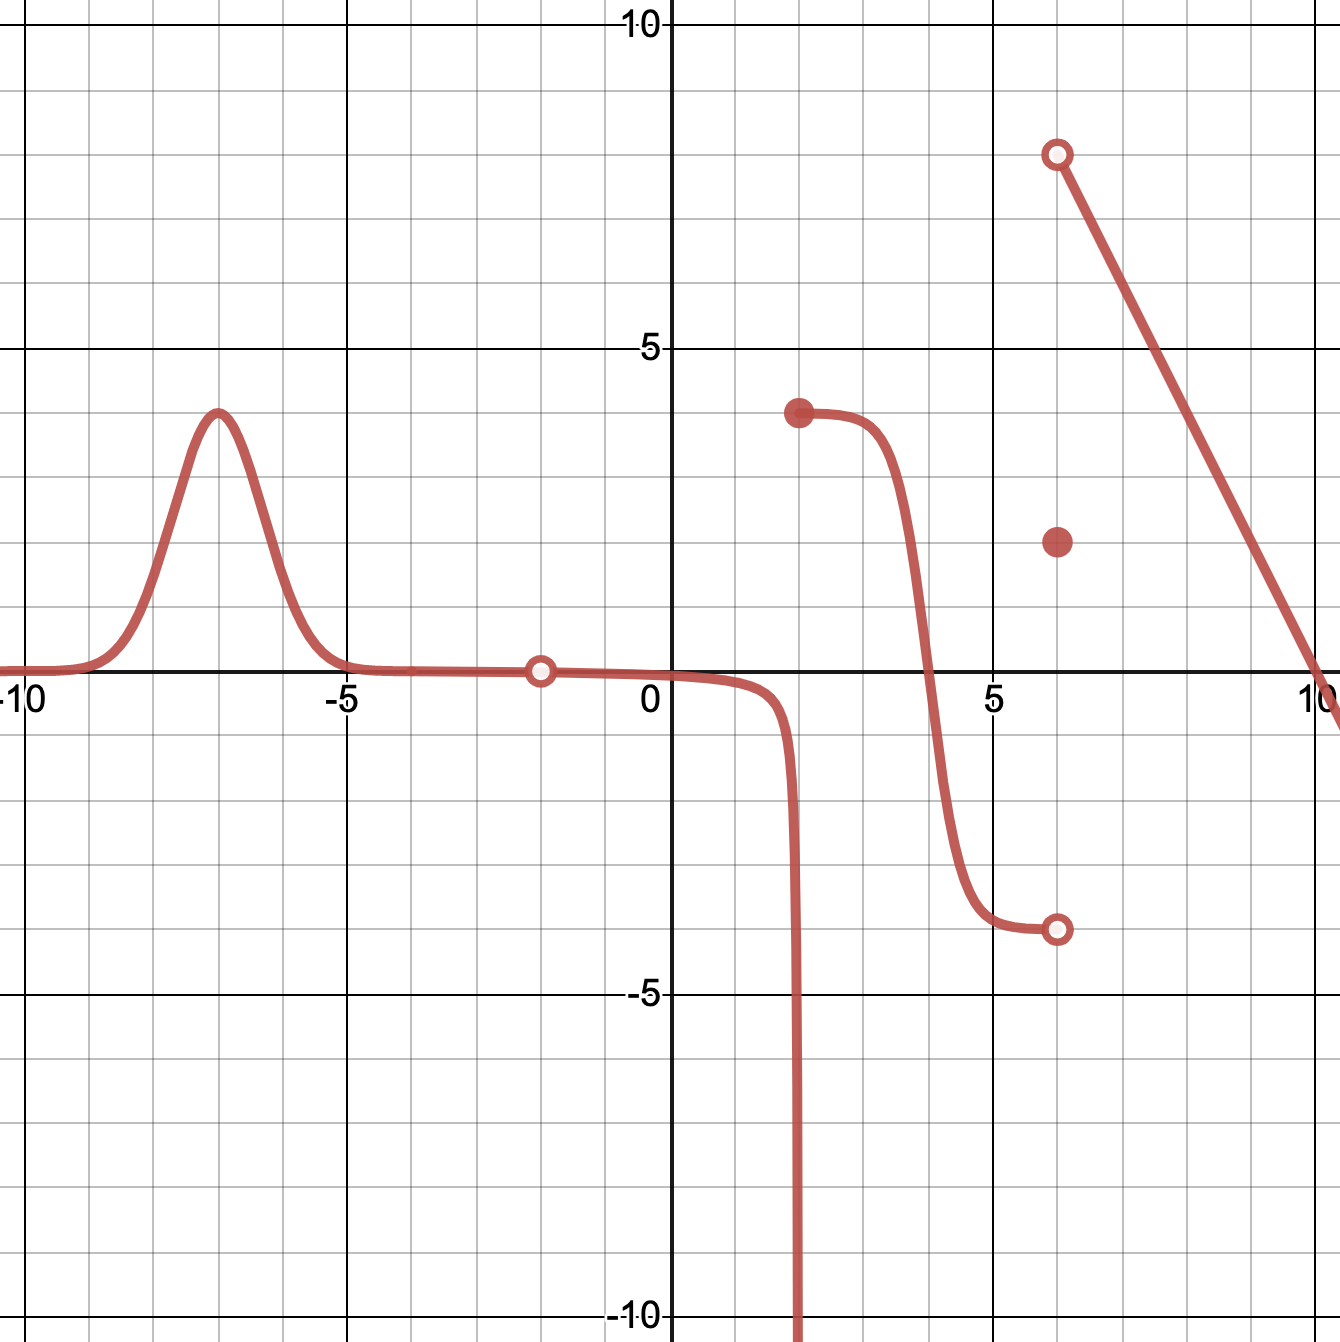
\includegraphics[width=0.5\linewidth]{img/pt1-graph2}
        \end{center}
    
        \begin{multicols}{4}
            \frq{$\lim\limits_{x\to-7}f(x)=$}
            \vspace{0.2cm}
            \frq{$\lim\limits_{x\to-7}f(x)=$}
            \vspace{0.2cm}
            \frq{$\lim\limits_{x\to-7}f(x)=$}
            \vspace{0.2cm}
            \frq{$f(-7)=$}
            \columnbreak
            
            \frq{$\lim\limits_{x\to-2}f(x)=$}
            \vspace{0.2cm}
            \frq{$\lim\limits_{x\to-2}f(x)=$}
            \vspace{0.2cm}
            \frq{$\lim\limits_{x\to-2}f(x)=$}
            \vspace{0.2cm}
            \frq{$f(-2)=$}
            \columnbreak
            
            \frq{$\lim\limits_{x\to2}f(x)=$}
            \vspace{0.2cm}
            \frq{$\lim\limits_{x\to2}f(x)=$}
            \vspace{0.2cm}
            \frq{$\lim\limits_{x\to2}f(x)=$}
            \vspace{0.2cm}
            \frq{$f(2)=$}
            \columnbreak
            
            \frq{$\lim\limits_{x\to6}f(x)=$}
            \vspace{0.2cm}
            \frq{$\lim\limits_{x\to6}f(x)=$}
            \vspace{0.2cm}
            \frq{$\lim\limits_{x\to6}f(x)=$}
            \vspace{0.2cm}
            \frq{$f(6)=$}
        \end{multicols}
    
    \begin{tabular}{c L{2cm} C{1cm} C{1cm} L{7cm}}
        & For & \multicolumn{2}{c}{Is $f(x)$ discontinuous?} & {If yes, what type of discontinuity exists at $x$?}\vspace{0.2cm} \\
        (q) & $x=-7$ & Y & N & \underline{\hspace{8cm}} \vspace{0.05cm} \\
        (r) & $x=-2$ & Y & N & \underline{\hspace{8cm}} \vspace{0.05cm} \\
        (s) & $x=2$ & Y & N & \underline{\hspace{8cm}} \vspace{0.05cm} \\
        (t) &  $x=6$ & Y & N & \underline{\hspace{8cm}} \vspace{0.05cm} 
    \end{tabular}

    At each of the following $x$-values, is $f(x)$ continuous, left-continuous, right-continuous, or neither?
    \begin{multicols}{4}
        \frq{x=-7}
        \frq{x=-2}
        \frq{x=2}
        \frq{x=6}
    \end{multicols}
    \end{multipartquestion}
    \newpage

    \begin{multipartquestion}
        Evaluate the following limits.
        \frq{$\lim\limits_{x\to1}\dfrac{x^2-2}{3x}$}
        \Smallsp
        \frq{$\lim\limits_{x\to3}\dfrac{x^2-9}{x^2-2x-3}$}
        \Smallsp
        \frq{$\lim\limits_{h\to0}\dfrac{\sqrt{7h+4}-2}{h}$}
        \Smallsp
        \frq{$\lim\limits_{\theta\to0}\dfrac{3\theta\cot(2\theta)}{5}$}
        \Smallsp
        \newpage
        \frq{$\lim\limits_{x\to3}\dfrac{x-1}{x^2-3}$}
        \Smallsp
        \frq{$\lim\limits_{x\to4}\dfrac{t^2-3t-4}{t^2-16}$}
        \Smallsp
        \frq{$\lim\limits_{x\to-1}\dfrac{\sqrt{x^2+8}-3}{x+1}$}
        \Smallsp
        \frq{$\lim\limits_{\theta\to0}\dfrac{3\tan(2\theta)}{4\theta}$}
        \Smallsp
        \newpage
        \frq{$\lim\limits_{x\to2}\dfrac{x-3}{16-x^2}$}
        \Smallsp
        \frq{$\lim\limits_{x\to3}\dfrac{x^3-9x}{x^2-x-6}$}
        \Smallsp
        \frq{$\lim\limits_{\theta\to0}3\csc(2\theta)\tan(2\theta)$}
        \Smallsp
        \frq{$\lim\limits_{x\to-3}\dfrac{x^2-9}{x^2-2x-15}$}
        \Smallsp
        \newpage
        \frq{$\lim\limits_{x\to-\infty}\dfrac{2x-\sqrt x}{x^2+2019}$}
        \Smallsp
        \frq{$\lim\limits_{x\to\infty}\left[\ln(3x+1)-\ln(2x+1)\right]$}
        \Smallsp
        \frq{$\lim\limits_{x\to-\infty}\dfrac{x^6-x^4+x^2-1}{7x^6+4x^3+10}$}
        \Smallsp
        \frq{$\lim\limits_{x\to\infty}\dfrac{\sqrt{7+9x^2}}{1-2x}$}
        \Smallsp
    \end{multipartquestion}
\end{document}